
\subsubsection{\textbf{2ºBucle:} \color{verdeOscuro}{\underline{Solución Óptima}}}

\par El segundo es el bucle exterior \texttt{for (size\_t i = 1; i < state.height - 1; ++i)}, es el mejor candidato para paralelizar, hay que añadir un
pragma \texttt{\#pragma omp parallel for reduction (+:difference)} para que ejecute las instrucciones en paralelo, pero teniendo en cuenta que la
instrucción, \texttt{difference = difference + abs (next\_state[ i ][ j ] - state[ i ][ j ]);}, no deben de ejecutarla dos hilos a la vez.

%%% TABLA DE TIEMPOS E IMÁGENES %%%
\begin{figure}[H]
    \centering
    \begin{subfigure}{0.4\textwidth}
        \begin{adjustbox}{width=\textwidth} 
        \begin{tabular}{|c|c|c|c|c|}
            \hline
            \rowcolor{azul} \multicolumn{2}{|c|}{}&\multicolumn{3}{c|}{\textbf{Compiler}} \\ \hline
            \rowcolor{azul} \multicolumn{2}{|c|}{}&\texttt{clang}&\texttt{gcc}&\texttt{icc}\\ \hline
            \rowcolor{azul} \textbf{Testing size} & \textbf{Threads}&\multicolumn{3}{c|}{\textbf{Average time (s)}} \\ \hline
            \multirow{8}{1cm}{\textbf{01-small}} & 1 & \(1.53\pm{0.00}\) & \(0.36\pm{0.00}\) & \(1.01\pm{0.01}\) \\ \cline{2-5}
            & 2 & \(0.81\pm{0.02}\) & \(0.18\pm{0.01}\) & \(0.53\pm{0.01}\) \\ \cline{2-5}
            & 3 & \(0.54\pm{0.00}\) & \(0.13\pm{0.01}\) & \(0.37\pm{0.00}\) \\ \cline{2-5}
            & 4 & \(0.42\pm{0.00}\) & \(0.12\pm{0.03}\) & \(0.34\pm{0.05}\) \\ \cline{2-5}
            & 5 & \(0.41\pm{0.01}\) & \(0.14\pm{0.01}\) & \(0.45\pm{0.01}\) \\ \cline{2-5}
            & 6 & \(0.35\pm{0.01}\) & \(0.13\pm{0.02}\) & \(0.40\pm{0.03}\) \\ \cline{2-5}
            & 7 & \(0.31\pm{0.01}\) & \(0.11\pm{0.00}\) & \(0.33\pm{0.01}\) \\ \cline{2-5}
            & 8 & \(0.29\pm{0.01}\) & \(0.11\pm{0.00}\) & \(0.33\pm{0.02}\) \\ \hline
        \end{tabular}
        \end{adjustbox}
    \end{subfigure}
    \hfill
    \begin{subfigure}{0.5\textwidth}
        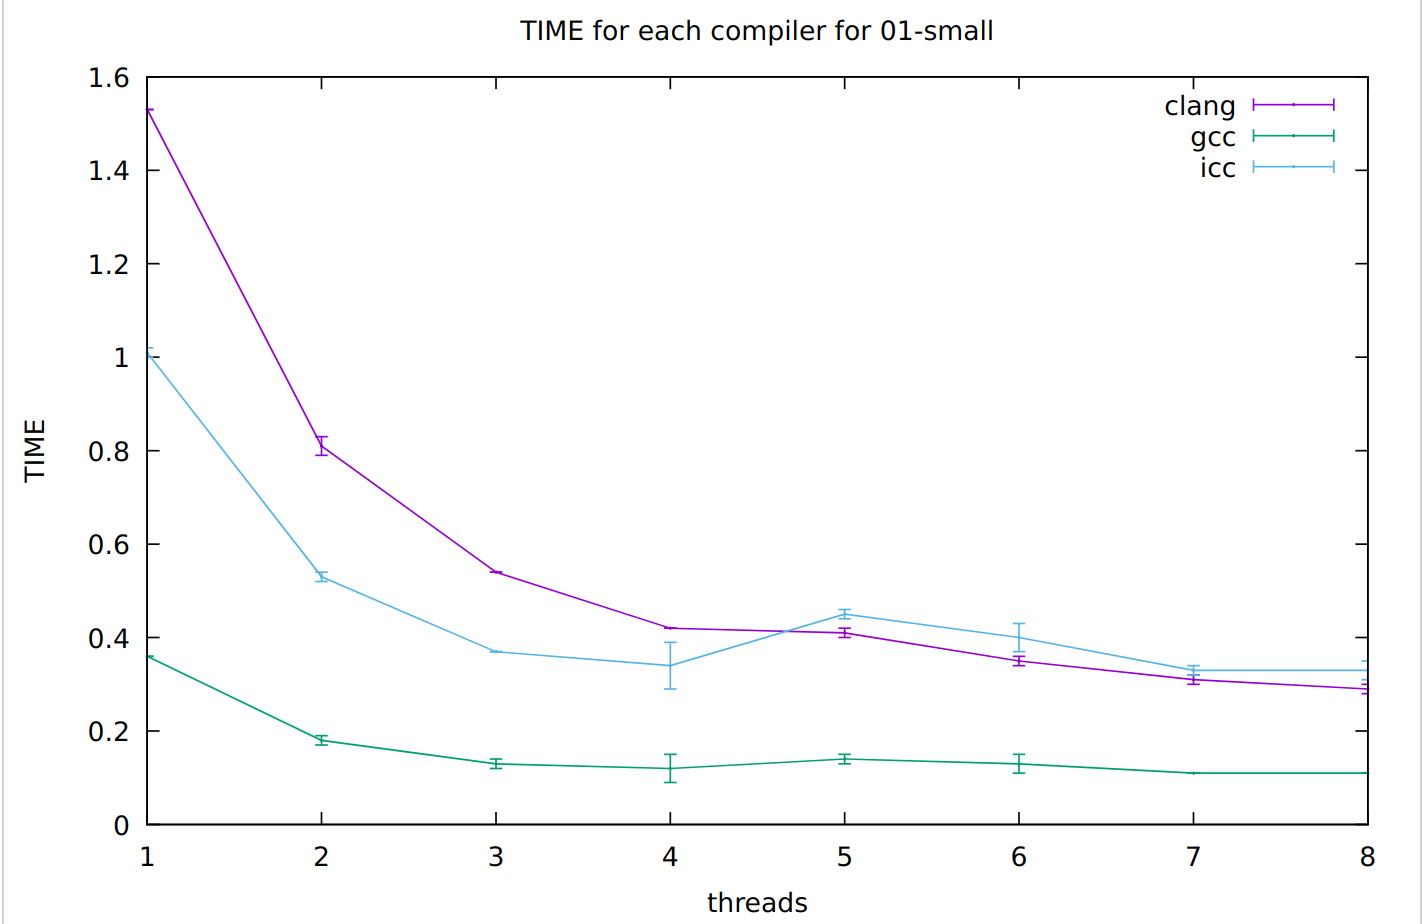
\includegraphics[width=\textwidth]{bucle2=01-small}
    \end{subfigure}
    \caption{\underline{2º Bucle, tamaño pequeño}: Tiempos de ejecución vs nº de hilos}
    \label{fig:bucle2=01-small}
\end{figure}

%%% TABLA DE TIEMPOS E IMÁGENES %%%
\begin{figure}[H]
    \centering
    \begin{subfigure}{0.4\textwidth}
        \begin{adjustbox}{width=\textwidth} 
        \begin{tabular}{|c|c|c|c|c|}
            \hline
            \rowcolor{azul} \multicolumn{2}{|c|}{}&\multicolumn{3}{c|}{\textbf{Compiler}} \\ \hline
            \rowcolor{azul} \multicolumn{2}{|c|}{}&\texttt{clang}&\texttt{gcc}&\texttt{icc}\\ \hline
            \rowcolor{azul} \textbf{Testing size} & \textbf{Threads}&\multicolumn{3}{c|}{\textbf{Average time (s)}} \\ \hline
            \multirow{8}{2.5cm}{\textbf{02-medium}} & 1 & \(4.45\pm{0.03}\) & \(0.89\pm{0.03}\) & \(2.90\pm{0.03}\) \\ \cline{2-5}
            & 2 & \(2.31\pm{0.05}\) & \(0.47\pm{0.02}\) & \(3.37\pm{0.06}\) \\ \cline{2-5}
            & 3 & \(1.52\pm{0.00}\) & \(0.33\pm{0.02}\) & \(2.93\pm{0.05}\) \\ \cline{2-5}
            & 4 & \(1.20\pm{0.03}\) & \(0.30\pm{0.06}\) & \(2.97\pm{0.03}\) \\ \cline{2-5}
            & 5 & \(1.16\pm{0.04}\) & \(0.37\pm{0.02}\) & \(2.96\pm{0.02}\) \\ \cline{2-5}
            & 6 & \(0.97\pm{0.03}\) & \(0.31\pm{0.01}\) & \(2.96\pm{0.07}\) \\ \cline{2-5}
            & 7 & \(0.87\pm{0.05}\) & \(0.27\pm{0.01}\) & \(2.93\pm{0.02}\) \\ \cline{2-5}
            & 8 & \(0.77\pm{0.03}\) & \(0.25\pm{0.01}\) & \(2.92\pm{0.01}\) \\ \hline
        \end{tabular}
        \end{adjustbox}
    \end{subfigure}
    \hfill
    \begin{subfigure}{0.5\textwidth}
        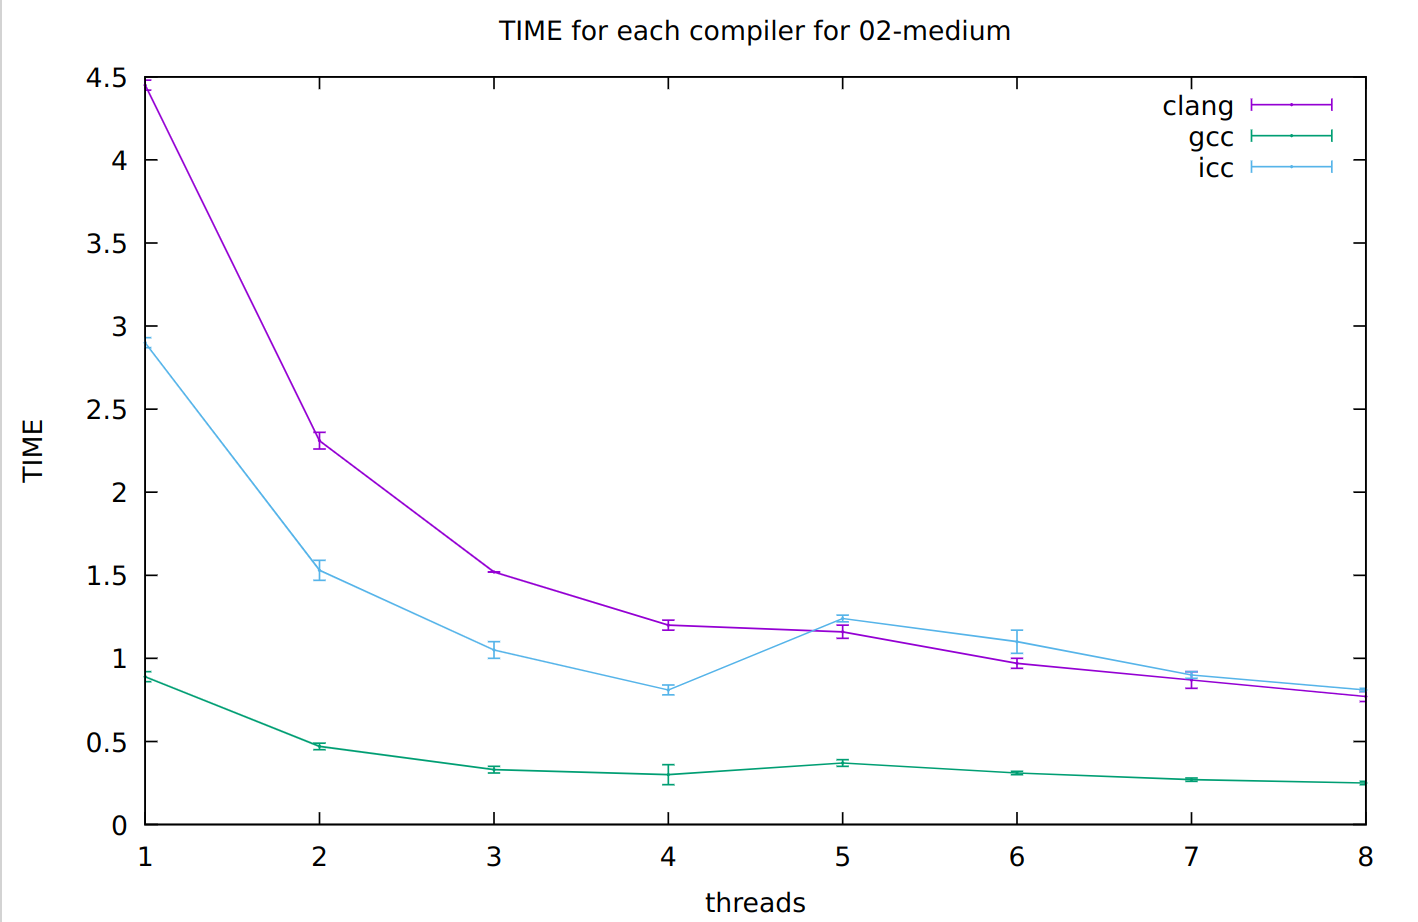
\includegraphics[width=\textwidth]{bucle2=02-medium}
    \end{subfigure}
    \caption{\underline{2º Bucle, tamaño mediano}: Tiempos de ejecución vs nº de hilos}
    \label{bucle2=02-medium}
\end{figure}

%%% TABLA DE TIEMPOS E IMÁGENES %%%
\begin{figure}[H]
    \centering
    \begin{subfigure}{0.4\textwidth}
        \begin{adjustbox}{width=\textwidth} 
        \begin{tabular}{|c|c|c|c|c|}
            \hline
            \rowcolor{azul} \multicolumn{2}{|c|}{}&\multicolumn{3}{c|}{\textbf{Compiler}} \\ \hline
            \rowcolor{azul} \multicolumn{2}{|c|}{}&\texttt{clang}&\texttt{gcc}&\texttt{icc}\\ \hline
            \rowcolor{azul} \textbf{Testing size} & \textbf{Threads}&\multicolumn{3}{c|}{\textbf{Average time (s)}} \\ \hline
            \multirow{8}{1cm}{\textbf{03-large}} & 1 & \(7.62\pm{0.15}\) & \(1.56\pm{0.07}\) & \(5.00\pm{0.12}\) \\ \cline{2-5}
            & 2 & \(3.93\pm{0.05}\) & \(0.80\pm{0.04}\) & \(2.63\pm{0.11}\) \\ \cline{2-5}
            & 3 & \(2.65\pm{0.02}\) & \(0.55\pm{0.04}\) & \(1.85\pm{0.15}\) \\ \cline{2-5}
            & 4 & \(2.02\pm{0.02}\) & \(0.42\pm{0.02}\) & \(1.37\pm{0.05}\) \\ \cline{2-5}
            & 5 & \(1.97\pm{0.12}\) & \(0.60\pm{0.03}\) & \(2.10\pm{0.02}\) \\ \cline{2-5}
            & 6 & \(1.67\pm{0.09}\) & \(0.51\pm{0.02}\) & \(1.78\pm{0.05}\) \\ \cline{2-5}
            & 7 & \(1.43\pm{0.07}\) & \(0.47\pm{0.04}\) & \(1.51\pm{0.02}\) \\ \cline{2-5}
            & 8 & \(1.28\pm{0.06}\) & \(0.41\pm{0.02}\) & \(1.40\pm{0.05}\) \\ \hline
        \end{tabular}
        \end{adjustbox}
    \end{subfigure}
    \hfill
    \begin{subfigure}{0.5\textwidth}
        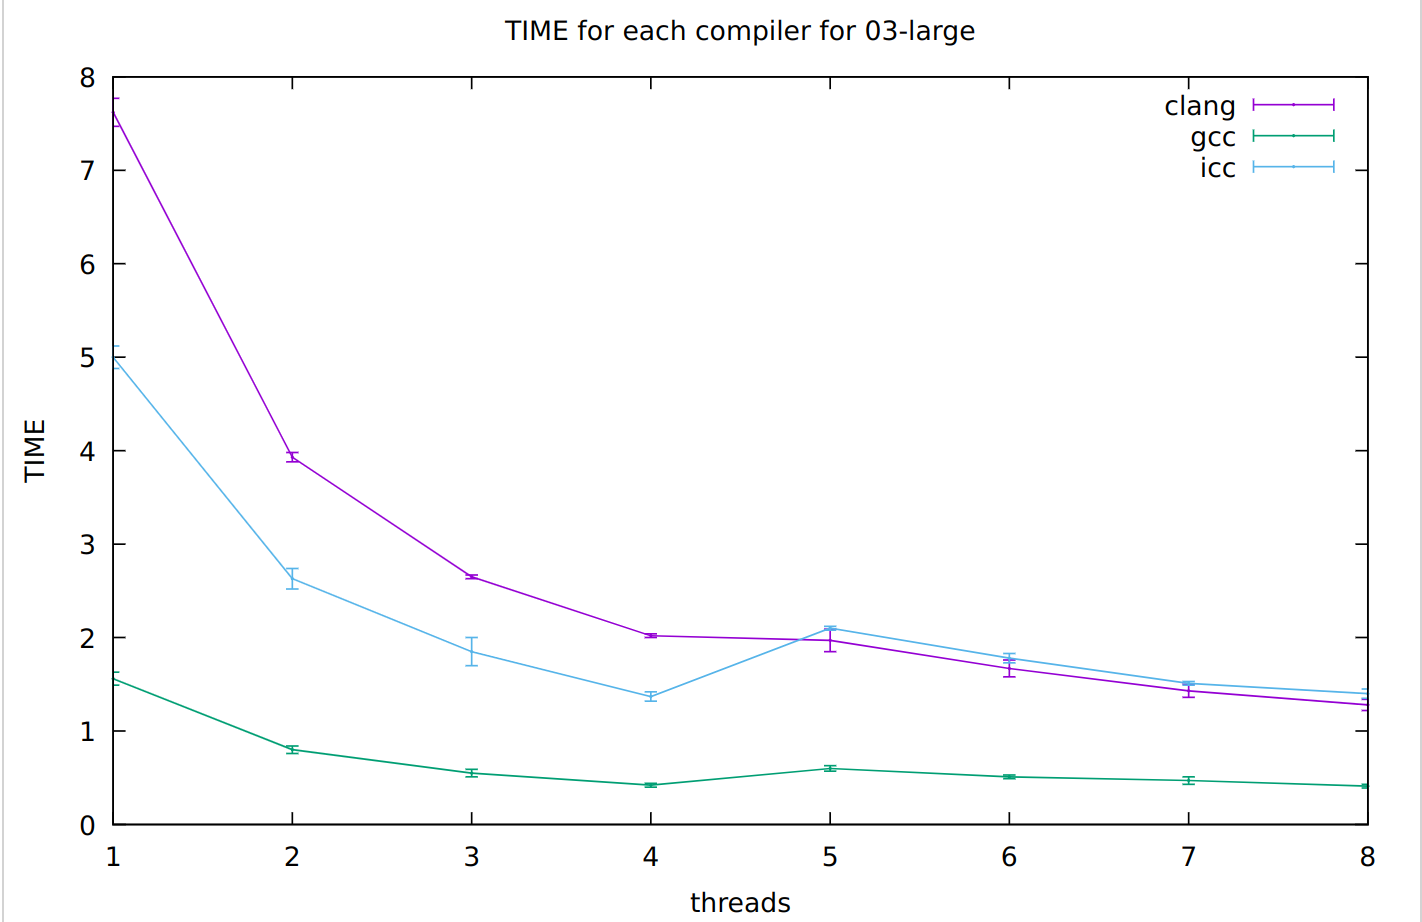
\includegraphics[width=\textwidth]{bucle2=03-large}
    \end{subfigure}
    \caption{\underline{2º Bucle, tamaño largo}: Tiempos de ejecución vs nº de hilos}
    \label{bucle2=03-large}
\end{figure}

\subsubsection{\textbf{heat.cpp}}
\begin{listing}[firstnumber=25]
    @@ -26,12 +26,13 @@   void solve() {
  + #pragma omp parallel for reduction (max:difference)
        for (size_t i = 1; i < state.height - 1; ++i) {
            for (size_t j = 1; j < state.width - 1; ++j) {
                next_state[i][j] = (state[i][j]
                                + state[i + 1][j]  
                                + state[i - 1][j]  
                                + state[i][j + 1]  
                                + state[i][j - 1]) / 5;
                difference = difference 
                             + abs(next_state[i][j]-state[i][j]);
            }
        }
\end{listing}
